\documentclass[onecolumn]{article}
%\usepackage{url}
%\usepackage{algorithmic}
\usepackage[a4paper]{geometry}
\usepackage{datetime}
\usepackage[margin=2em, font=small,labelfont=it]{caption}
\usepackage{graphicx}
\usepackage{mathpazo} % use palatino
\usepackage[scaled]{helvet} % helvetica
\usepackage{microtype}
\usepackage{amsmath}
\usepackage{subfigure}
\usepackage{hyperref}
\usepackage{graphicx}


\usepackage{listings}
\usepackage{color}
\definecolor{dkgreen}{rgb}{0,0.6,0}
\definecolor{gray}{rgb}{0.5,0.5,0.5}
\definecolor{mauve}{rgb}{0.58,0,0.82}

\lstset{frame=tb,
  language=python,
  aboveskip=3mm,
  belowskip=3mm,
  showstringspaces=false,
  columns=flexible,
  basicstyle={\small\ttfamily},
  numbers=none,
  numberstyle=\tiny\color{gray},
  keywordstyle=\color{blue},
  commentstyle=\color{dkgreen},
  stringstyle=\color{mauve},
  breaklines=true,
  breakatwhitespace=true,
  tabsize=2
}

% Letterspacing macros
\newcommand{\spacecaps}[1]{\textls[200]{\MakeUppercase{#1}}}
\newcommand{\spacesc}[1]{\textls[50]{\textsc{\MakeLowercase{#1}}}}

\title{\spacecaps{CENG 3521 Data Mining Assigment 1 }\\ \normalsize \spacesc{} }

\author{Gizem PESEN\\pesengizem@gmail.com}

%\date{\today\\\currenttime}


\begin{document}
\maketitle



\section{Contents }

\begin{itemize}
\item \hyperref[sec:1]{Declaration of Honor Code}
\item \hyperref[sec:2]{Regression Task}
\item \hyperref[sec:2]{Curse of dimensionality}
\item \hyperref[sec:2.0.1]{Generate Test Datasets in Python with scikit-learn}
\item \hyperref[sec:2.0.2]{Training and Testing}
\item \hyperref[sec:2.0.3]{ SGD and Linear Regression }   
\item \hyperref[sec:2.0.4]{Discussion }  
\item  \hyperref[sec:2.0.5]{Sampling and dimensionality reduction}
\item \hyperref[sec:2.0.6]{Principal Component Analysis (PCA)}
\item \hyperref[sec:3]{ Classification Task}
\item \hyperref[sec:3.0.1]{Visualization and binary-class classification}
\end{itemize}

.\\\\\\\\\\\\\\
\section{Declaration of Honor Code}
\label{sec:1}
\textbf{Student ID :}170709050\\
\textbf{Name Surname:}Gizem Pesen\\

In the course of Data Mining (CENG 3521), I take academic integrity very seriously and ask
you to do as well. That’s why, this page is dedicated to some clear statements that defines
the policies of this assignment, and hence, will be in force. Before reading this assignment
booklet, please first read the following rules to avoid any possible violation on academic
integrity.
\\
\begin{itemize}
\item This assignment must be done individually unless stated otherwise.
\item You are encouraged to discuss with your classmates about the given assignments, but
these discussions should be carried out in an abstract way. That is, you cannot copy
code (in whole or in part) of someone else, cannot share your code (in whole or in part)
with someone else either.
\item The previous rule also holds for the material found on the web as everything on the web
has been written by someone else.
• You must not look at solution sets o
\item You must not look at solution sets or program code from other years.
\item You cannot share or leave your code (in whole or in part) in publicly accessible areas.
\item You have to be prepared to explain the idea behind the solution of this assignment you
submit.
\item Finally, you must make a copy of your solution of this assignment and keep it until the
end of this semester.

\end{itemize}
\begin{figure}[ht!]
\centering

\includegraphics[width=10cm]{img3.png}
\end{figure}




\section{Regression Task}
\label{sec:2}

\section{Curse of dimensionality}
\label{sec:2}

\subsubsection{ Generate Test Datasets in Python with scikit-learn}
\label{sec:2.0.1}

Test datasets are small contrived datasets that let you test a machine learning algorithm or test harness.\\ The scikit-learn Python library provides a suite of functions for generating samples from configurable test problems for regression and classification.

\begin{lstlisting}[language=Python, caption=generate data] 
m = 10000
n = 100
X, y = make_regression(n_samples=m, n_features=n, noise=0.1)
\end{lstlisting} 

\begin{figure}[ht!]
\centering
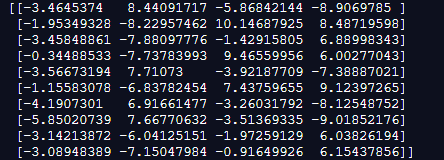
\includegraphics[width=5cm]{img2.png}
\caption{Output \label{}}
\end{figure}

\subsubsection{Training and Testing}
\label{sec:2.0.2}
Train/Test is a method to measure the accuracy of your model.It is called Train/Test because you split the the data set into two sets: a training set and a testing set.\\
\begin{figure}[ht!]
\centering
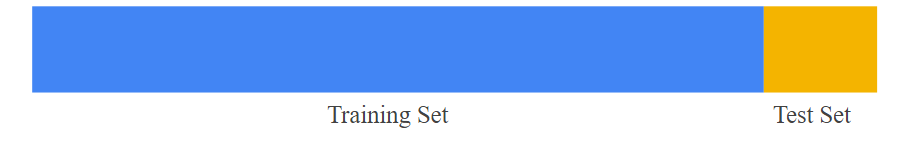
\includegraphics[width=5cm]{img1.png}
\caption{Training and Testing \label{}}
\end{figure}
Separating data into training and testing sets is an important part of evaluating data mining models. Typically, when you separate a data set into a training set and testing set, most of the data is used for training, and a smaller portion of the data is used for testing.

\begin{lstlisting}[language=Python, caption=train and test] 
X_train, X_test, y_train, y_test = train_test_split(X, y, test_size=0.33, random_state=42)
\end{lstlisting} 

\subsubsection{Stochastic Gradient Descent and Linear Regression}
\label{sec:2.0.3}
Gradient Descent is the process of minimizing a function by following the gradients of the cost function.\\
In machine learning, we can use a technique that evaluates and updates the coefficients every iteration called stochastic gradient descent to minimize the error of a model on our training data.

\begin{lstlisting}[language=Python, caption=train and test] 
n_iter=1000 #with 1,000 iterations

start = time.time() #calculate training time
clf = SGDRegressor(max_iter=n_iter)
clf.fit(X_train,y_train)#train the model or fits a linear model
\end{lstlisting} 

And below you can see the calculation of error:

\begin{lstlisting}[language=Python, caption=Prediction test] 
prediction_test = clf.predict(X_test)  # make a prediction
print("Error =",mean_squared_error(y_test,prediction_test))
\end{lstlisting} 

\subsubsection{Discussion}
\label{sec:2.0.4}

\begin{enumerate}
\item It is positive relation between dimension size and training time and error.
\item It is  negative relation between tuple size and error yield by the algorithm.
\item It is positive relation between tuple size and training time.

\end{enumerate}
\begin {tabular}{crrrrl}
\hline
Tuple Size (m)& Dimension Size (n)  &Training Time (in ms))
& Error (cost)
  \\
\hline
  10,000& 100
& 0.10&5.2\\
 10,000& 1,000
 &0.25&9.5 \\
 10,000& 2,000
& 0.50&2.0\\ 
\hline
\end{tabular}
\\\\

\begin {tabular}{crrrrl}
\hline
Tuple Size (m)& Dimension Size (n)  &Training Time (in ms))
& Error (cost)
  \\
\hline
  100,000& 
100&0.38&1.2\\ 250000
 &100
 &0.70&2.4\\
 500000&100
&1.25& 2.05\\
\hline
\end{tabular}
\\

\section{ Sampling and dimensionality reduction}
\label{sec:3}


\subsubsection{Principal Component Analysis (PCA)  }
\label{sec:3.0.1}

\begin{lstlisting}[language=Python, caption=load a dataset from sklearn module] 
pca = PCA(n_components=2)
pca.fit(X)
print(pca.explained_variance_ratio_)
print(pca.singular_values_)
\end{lstlisting} 
.\\\\
\section{Classification Task}
\label{sec:3}

\subsubsection{Visualization and binary-class classification}
\label{sec:3.0.1}

\begin{lstlisting}[language=Python, caption=extra libraries] 
from sklearn.datasets import make_moons
from matplotlib import pyplot
from pandas import DataFrame
from sklearn.linear_model import LogisticRegression 
\end{lstlisting} 

\begin{lstlisting}[language=Python, caption=load a dataset from sklearn module] 
X, y = make_moons(n_samples=100, noise=0.1)
\end{lstlisting} 

\begin{lstlisting}[language=Python, caption= training and testing] 
X_train, X_test, y_train, y_test = train_test_split(X, y, test_size=0.3, random_state=42)
\end{lstlisting} 

\begin{lstlisting}[language=Python, caption= logistic regression algorithm with SGD solver] 
clf = LogisticRegression().fit(X_test[:100], y_test[:100])
\end{lstlisting} 

\begin{figure}[ht!]
\centering
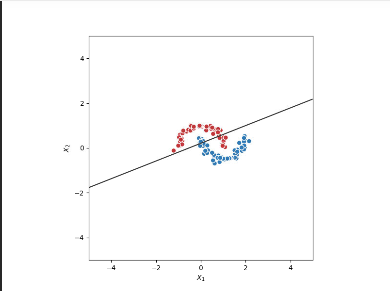
\includegraphics[width=3cm]{moon.png}
\caption{Output \label{}}
\end{figure}

\begin{lstlisting}[language=Python, caption= logistic regression 
xx, yy = np.mgrid[-5:5:.01, -5:5:.01]
grid = np.c_[xx.ravel(), yy.ravel()]
probs = clf.predict_proba(grid)[:, 1].reshape(xx.shape)

f, ax = plt.subplots(figsize=(8, 6))
ax.contour(xx, yy, probs, levels=[.5], cmap="Greys", vmin=0, vmax=.6)

ax.scatter(X[:,0], X[:, 1], c=y, s=50,
           cmap="RdBu", vmin=-.2, vmax=1.2,
           edgecolor="white", linewidth=1)

ax.set(aspect="equal",
       xlim=(-5, 5), ylim=(-5, 5),
       xlabel="$X_1$", ylabel="$X_2$")

\end{lstlisting} 





 
\nocite{*}
\bibliographystyle{plain}
\bibliography{references}
\end{document}
